\setlength{\parindent}{4em}
\setlength{\parskip}{1em}

O nosso projeto consiste em um serviço de bate papo online, que possui, além do chat online, a opção de criar salas de reunião. A implementação do sistema foi feita em Java, aproveitando os códigos do Zookeeper que vimos em aula.\par
Para ligar o chat, faz-se necessário configurar o Zookeeper na máquina (como feito nas aulas práticas) e executar o arquivo ClientCLI.java. Esse arquivo é responsável por organizar o ambiente de usuário de maneira intuitiva, afim de facilitar a interação entre o usuário e o sistema. Dentro da CLI, o usuário tem as seguintes opções de comando:
\begin{itemize}
	\item entrar
	\par Entra numa sala de reunião.
	\item criar
	\par Cria uma sala de reunião nova.
	\item sair
	\par Sai da sala de reunião atual.
	\item ajuda
	\par Lista os comandos possíveis de serem executados e como usá-los.
	\item enviar
	\par Envia mensagem num chat individual ou reunião.
	\item receber
	\par Primeiro faz a busca de mensagens antigas (enviadas antes do usuário fazer login) e depois fica esperando a notificação de mensagens novas.
	\item parar
	\par Comando para parar de esperar a notificação de mensagens novas.
	\item transmitir
	\par Inicia a transmissão de conteúdo dentro da sala de reunião.
	\item chat
	\par Especifica o tipo de mensangem que o usuário quer enviar.
	\item reuniao
	\par Especifica o tipo de sala que o usuário quer se conectar.
\end{itemize}
\par
Aqui está a representação de uma sala chat funcionando. Fazemos o login com 4 usuários diferentes e fazemos 3 deles enviar uma mensagem para o mesmo usuário ("mario"). Ele aguarda o recebimento das mensagens e é notificado:
\begin{center}
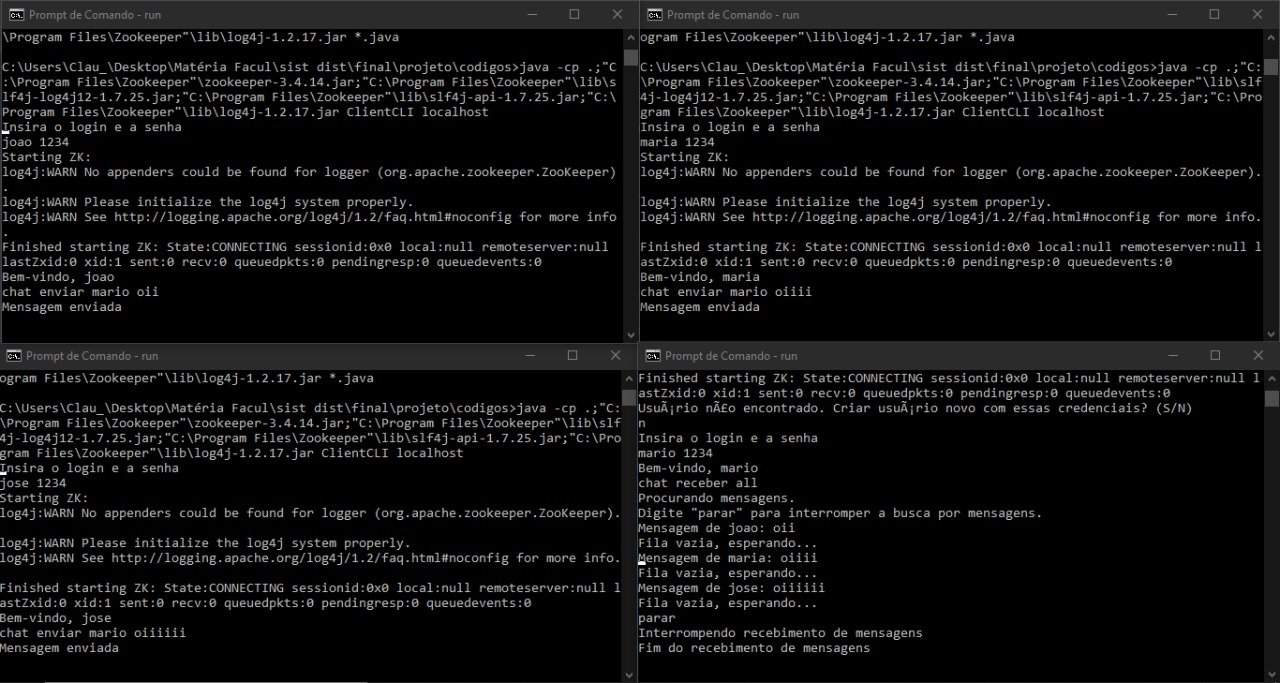
\includegraphics[width=20cm]{projeto/prints/exemplo-chat1.jpeg}
\end{center}

\par Exemplo de reunião. O primeiro usuário cria a sala de reunião e ele é o líder da sala. Os demais conectam na sala e o líder inicia a sua apresentação. Quando o líder sai da sala, um novo líder é eleito e esse novo líder pode iniciar sua apresentação.

\begin{center}
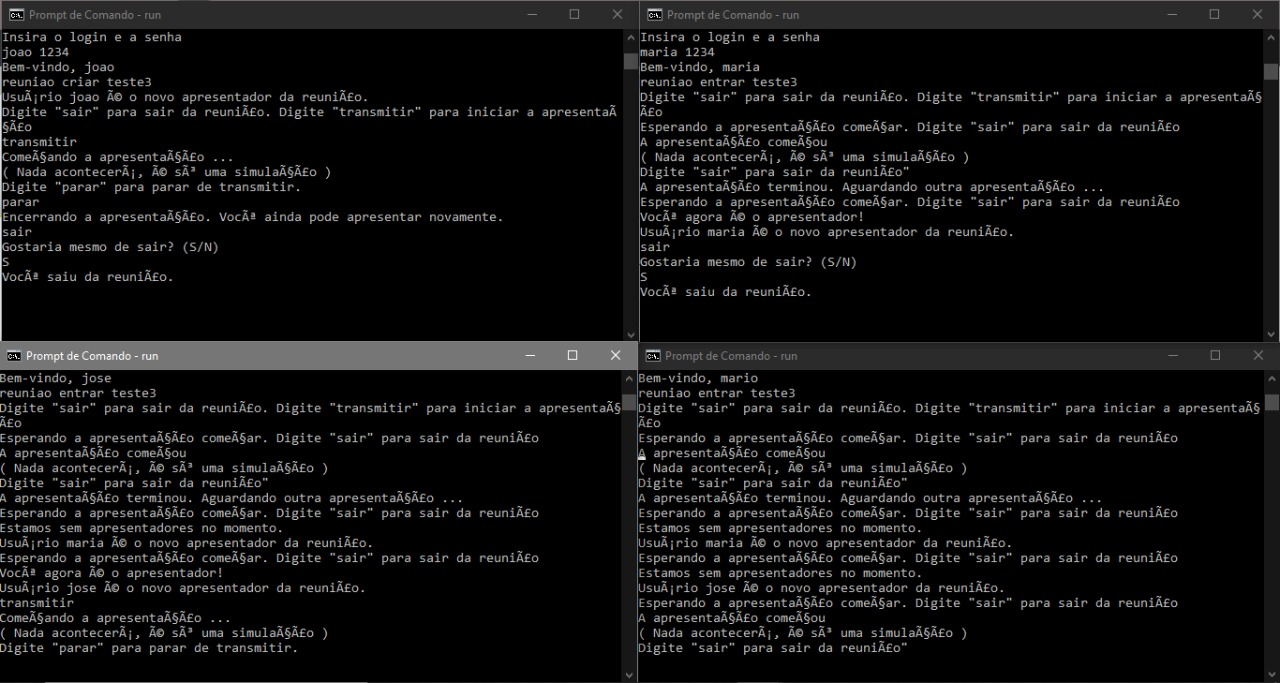
\includegraphics[width=20cm]{projeto/prints/exemplo-reuniao1.jpeg}
\end{center}
